\chapter{Introduction}
\label{chapter:introduction}
\section{Mathematical Finance}
\label{section:mathematical finance}
Mathematical finance, also known as quantitative finance, is a field of applied mathematics focused on the modeling of financial instruments.
It is rather difficult to overestimate its importance since it is heavily used by investors and investment banks in everyday transactions.
In recent decades, this field suffered a complete paradigm shift, following developments in computer science and new theoretical results that enabled investors to better understand the mechanics of financial markets.

With the colossal sums traded daily in financial markets around the world, mathematical finance has become increasingly important and many resources are invested in the research and development of new and better theories and algorithms.


\section{Derivatives}
\label{section:derivatives}
Derivatives are currently one of the subjects most studied by financial mathematicians.
In finance, a \emph{derivative} is simply a contract whose value depends on other simpler financial instruments, known as \emph{underlying assets}, such as stock prices or interest rates.
They can virtually take any form desirable, so long as there are two parties interested in signing it and all government regulations are met.


The importance of derivatives has grown greatly in recent years. In fact, as of June 2017, derivatives were responsible for over \textdollar542 trillion worth of trades, in the Over-the-Counter (OTC) market alone~\cite{BIS}, as can be seen in \autoref{fig:OTC} (the OTC market refers to all deals signed outside of exchanges).
This growth stalled after the 2008 global financial crisis due to new government regulations, implemented because of the role of derivatives in the market crash~\cite{FT}. It is easy to see that mishandling derivatives can have disastrous consequences. However, when handled appropriately, derivatives prove to be very powerful tools to investors, as we will see.


\begin{figure}[!htb]
    \centering
      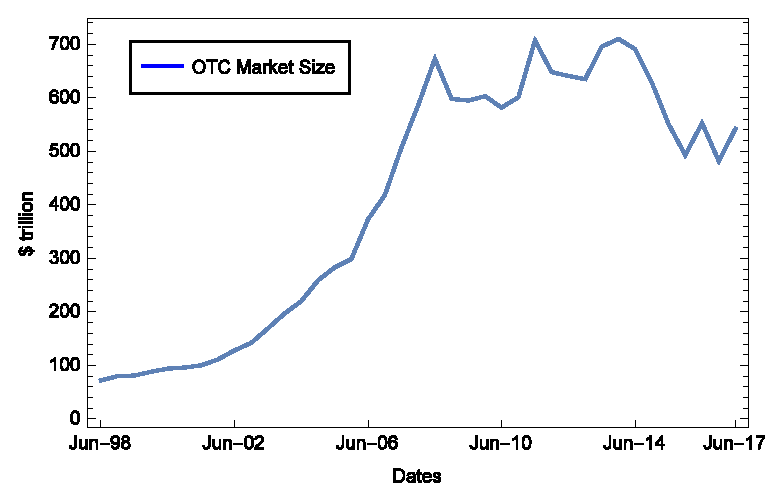
\includegraphics[width=.6\linewidth,trim={2pt 17pt 0 0},clip]{OTC.eps}
      \caption{Size of OTC derivatives market since May 1996.}\label{fig:OTC}
    \end{figure}

\section{Options}
\label{section:options}
Of all kinds of derivatives, in this master thesis we will focus particularly on the most traded type~\cite{Hull}: \emph{options}.

As the name implies, an \emph{option} contract grants its buyer the option to buy (in the case of a \emph{call} type option) or sell (for \emph{put} options) its underlying asset at a future date, known as the \emph{maturity}, for a fixed price, known as the \emph{strike price}.
In other words, when signing an option, buyers choose a price at which they want to buy/sell (call/put) some asset and a future date to do this transaction. When this date arrives, if the transaction is favorable to the buyers, they exercise their right to execute it.

The description above pertains only to the most traded type of option - \emph{European} options. In this thesis, unless otherwise stated, all options will be assumed European. There exist, however, other option types that enable exercising at dates other than maturity.
The most well known such example is \emph{American} options, contracts that enable their buyers to exercise their right to buy/sell the underlying asset at any point in time \emph{until} the maturity date.
Other types, commonly known as \emph{Exotic} options, will be studied in more detail in the following sections.

%The two main types of options are calls and puts. They grant their buyer the right to buy and sell the underlying asset, respectively, for a fixed price, known as the strike price, in the future.

It's important to emphasize the fact that an option grants its buyer the right to do something. If \emph{exercising} the option would lead to losses, the buyer can simply decide to let the maturity date pass, allowing the option to expire without further investments. This is indeed the most attractive characteristic of options.


\iffalse
\subsection{European and American Options}
\label{subsection:european and american options}
Options are also categorized by the period at which the buyer is allowed to exercise his right. The two most traded types are European and American options.
With an European option, an investor is only able to exercise the contract at the expiration date. The value of the underlying asset up to that point in time is irrelevant.
As for American options, the buyer can exercise the contract at any moment up to the expiration date.
In this case, the investor is faced with an optimal-stopping problem: when is the best time to exercise the option?
For this very reason, it should be clear that American options are significantly more difficult to study than their European counterparts.
\fi

\subsection{Why Options are Important}
\label{subsection:why options are important}
Options are very useful tools to all types of investors. 

To hedgers (i.e. investors that want to limit their exposure to risk), options provide safety by fixing a minimum future price on their underlying assets - e.g. if hedgers want to protect themselves against a potential future price crash affecting one of their assets, they can buy put type options on that asset. With these, even if the asset's value does crash, their losses will always be contained because they can exercise the options and sell the asset at the option's higher strike price.

Options are also very useful to speculators (i.e. investors that try to predict future market movements). The lower price of options (when compared to their underlying assets) grants this type of investors great leveraging capabilities and, with them, access to much higher profits if their predictions prove true. The opposite is also true and a wrong prediction can equally lead to much greater losses.

Due to all their advantages, and unlike some other types of derivatives, options have a price. Finding the ideal price for an option is a fundamental concern to investors, because knowing the appropriate value of an option can give them a chance to take advantage of under or overpriced options.
Finding this price can be very difficult for some options, however. Though a lot of research has been done towards this goal, a great deal more is still required.

